% !TeX encoding = UTF-8
% !TeX program = pdflatex
% !BIB program = biber
% rubber: setlist arguments --shell-escape

% Template Revision:
% Rev  E1 -- 2021-12    -- Simone Atzwanger
% Rev. D1 -- 2021-06    -- Max Heisinger
% Rev. C2 -- 2021-05-11 -- Ali Varli
% Rev. C1 -- 2021-03-22 -- Ali Varli
% Rev. B1 -- 2019-11-05 -- Ali Varli

\documentclass[%
	a4paper,
	11pt,
	BCOR=10mm,
	DIV=12,
	headinclude,
	headheight=16mm,
	oneside,
	onecolumn,
	openany,
	parskip=half,
	% appendixprefix,
	% toc=flat,
	% chapterentrydots=true,
    chapterprefix,
	table,
	fleqn,
	% draft
]{scrbook}[2015/09/29]% needs version 3.19 or newer

\usepackage[utf8]{inputenc}

% !TeX encoding = UTF-8
% !TeX root = MAIN.tex

\newif\ifeng
%% HINWEISE: Hier müssen folgende Einstellungen vorgenommen werden:
%% PLEASE NOTE: Select your settings here:

%% Sprache: Falls die Dokumentensprache Deutsch ist, \engtrue mit einem %-Zeichen davor auskommentieren:
%% Language: If the document language is German, comment \engtrue with a % sign in front:
\engtrue

%% Hier den Namen des Autors eingeben:
%% Enter the author’s name here:
%TODO change name
\def\author{Mohamad Khabour}

%% Hier Informationen für den rechten Block unter dem JKU-Logo eingeben, wobei die Elemente mit einem Buchstaben jeweils für die Beschreibung und mit Doppelbuchstaben für den Inhalt sind.
%% Anzuführen bei Masterarbeit: Eingereicht von, Anfegertigt am, BeurteilerIn, Mitbetreuung.
%% Anzuführen bei Dissertation: Eingereicht von, Anfegertigt am, ErstbeurteilerIn, ZweitbeurteilerIn, Mitbetreuung.
%% Anzuführen bei strukturiertem Doktorat: Eingereicht von, Angefertigt am, ErstbetreuerIn, ZweitbetreuerIn, Mitbetreuung.
%%
%% Enter information here for the right block under the JKU logo, whereby the elements should have one letter for the heading and double letters for content.
%% To be given for master thesis: Author, Submission, Thesis Supervisor, Assistant Thesis Supervisor.
%% To be given for doctoral thesis: Author, Submission, First Supervisor, Second Supervisor, Assistant Thesis Supervisor.
%TODO change degree and matriculation number
\def\elementA{Author}
\def\elementAA{\textbf{\author} Bachelor of Science \\ k12005283}

%TODO change the name of the institute
\def\elementB{Submission}
\def\elementBB{\textbf{Institut für Symbolic Artificial Intelligence}}

%TODO change name of supervisor
\def\elementC{Supervisor}
\def\elementCC{Univ.-Prof.\textsuperscript{in} Dr.\textsuperscript{in}\@ \textbf{Martina Seidl}}

%TODO optional second supervisor
%\def\elementD{Assistant Thesis Supervisor}
%\def\elementDD{Prof.~Dr.\@ \textbf{Firstname Lastname}}

%TODO add your own finish date
%% Hier Datum eingeben (Monat der Abgabe im Prüfungs- und Anerkennungsservice):
%% Enter the date (Month and year of submission to Examination and Recognition Services):
\def\date{May 2026}

%TODO add your location
%% Hier Ort eingeben:
%% Enter the location:
\def\place{Linz}

%TODO add the title of your work
%% Hier Titel eingeben; steht über dem K:
%% Enter the title; it appears above the K:
\def\title{Systematic Testing of QBF Solvers via Truth-Value-Preserving Transformations}

%% Hier den Typ der Arbeit eingeben (0: Keine Arbeit, 1: Bachelorarbeit, 2: Masterarbeit, 3: Dissertation, 4: Diplomarbeit):
%% Enter the type of paper here (0: Not Thesis, 1: Bachelor’s Thesis, 2: Master’s Thesis, 3: Dissertation, 4: Diploma Degree Thesis):
\def\type{1}

%% Hier ggf. Untertitel eingeben; stehen unter dem K (nur bei 0):
%% If necessary, enter a subtitle here; below the K (only for 0):
%% \def\subtitle{Subtitle / Untertitel}

%TODO change degree (Computer Science: Diplom-Ingenieur or Diplom-Ingenieurin; AI: Master of Science)
%% Hier den angestrebten akademischen Grad eingeben:
%% Enter the desired academic degree here:
\def\acadDegree{Bachelor of Science (BSc)}

%TODO add your filed of study (Computer Science or Artificial Intelligence)
%% Hier die Studienrichtung eingeben:
%% Enter the major here:
\def\study{Computer Science}


%TODO add all the metadata info
%% Hier die Metadaten für das PDF eingeben (mehrere Autoren und Keywords durch \sep trennen):
%% Enter metadata for the PDF here (seperate multiple authors and keywords by \sep):
\begin{filecontents*}[overwrite]{\jobname.xmpdata}
\Title{Systematic Testing of QBF Solvers via Truth-Value-Preserving Transformations}
\Author{Mohamad Khabour}
\Subject{Bachelor Thesis}
\Keywords{a, b, c, d}
\Language{en-US}
\Publisher{}
\end{filecontents*}

%%% Local Variables: 
%%% TeX-master: "main"
%%% TeX-engine: default
%%% TeX-command-extra-options: "-shell-escape"
%%% End: 


\usepackage{pdfpages}
\usepackage[T2A]{fontenc}
\usepackage{mathpazo}
\usepackage[nottdefault]{sourcecodepro}
\usepackage[bitstream-charter]{mathdesign}
\usepackage{microtype}
\DisableLigatures{encoding = *, family = tt* }
\usepackage[scale=0.97]{XCharter}
\setkomafont{disposition}{\bfseries}
\ifeng%
	\usepackage[ngerman,english]{babel}
\else
	\usepackage[english,ngerman]{babel}
\fi
\usepackage[absolute]{textpos}
\usepackage[binary-units]{siunitx}
\usepackage{amsmath}
\usepackage[%
	backend=biber,
	style=numeric-comp, % authoryear
	bibstyle=numeric, % authoryear
	citestyle=numeric, % authoryear
	% maxcitenames=2,
	sorting=none, %nty
	backref=true,
	backrefstyle=none
]{biblatex}
\addbibresource{literature.bib}
\usepackage{csquotes}
\usepackage{lastpage,scrlayer-scrpage}
\usepackage{seqsplit}
\pagestyle{scrheadings}
\clearpairofpagestyles%

\ifeng%
	\ohead*{
\includegraphics[width=3cm]{cover/jkuen}}
\else
	\ohead*{
\includegraphics[width=3cm]{cover/jkude}}
\fi

\ifoot*{\date}
\cfoot*{\author}
\ofoot*{\pagemark/\pageref{LastPage}}

\setkomafont{pageheadfoot}{\sffamily\scriptsize}
\setkomafont{pagenumber}{\sffamily\scriptsize}

\usepackage[onehalfspacing]{setspace}
\usepackage{booktabs,colortbl,xcolor}
\usepackage{graphicx,wrapfig}
\graphicspath{{images/}}
\usepackage[section]{placeins} %\FloatBarrier
\usepackage{float} %[H]
\usepackage{enumitem}
\usepackage{subfiles}
\usepackage{scrhack}
\usepackage[%
	bookmarksnumbered=true,
	pdfborder={0 0 0},
	pdfa
]{hyperref}
\usepackage[super]{nth}
\usepackage{subfigure}

\usepackage[newfloat]{minted}
\usemintedstyle{friendly}
\usepackage{caption}
\usepackage{mwe}
\newenvironment{code}{\captionsetup{type=listing}}{}
\SetupFloatingEnvironment{listing}{name=Listing}

% from http://tex.stackexchange.com/questions/57151/how-do-i-prevent-conflicts-between-accsupp-and-hyperref
\usepackage{accsupp}
\newcommand\emptyaccsupp[1]{\BeginAccSupp{ActualText={}}#1\EndAccSupp{}}


%default definition is: \def\theFancyVerbLine{\rmfamily\tiny\arabic{FancyVerbLine}}
\let\theHFancyVerbLine\theFancyVerbLine% don't apply our patch to hyperref's version
\def\theFancyVerbLine{\rmfamily\tiny\emptyaccsupp{\arabic{FancyVerbLine}}}

%% Taken from https://tex.stackexchange.com/a/35494
\newenvironment{longdescription}
  {\begin{description}[style=unboxed]}
  {\end{description}}

\usepackage{cmap}
\usepackage[a-2b]{pdfx}
\usepackage{colorprofiles}

\usepackage{tikz}

%% Example for diagrams taken from https://texample.net/tikz/examples/android/
\usetikzlibrary{arrows,arrows.meta,calc,shapes,automata}
\usetikzlibrary{positioning}
\tikzset{%
  >={Latex[width=2mm,length=2mm]},
  % Specifications for style of nodes:
            base/.style = {rectangle, rounded corners, draw=black,
                           minimum width=4cm, minimum height=1cm,
                           text centered, font=\sffamily},
          starts/.style = {base, fill=blue!30},
           stops/.style = {base, fill=red!30},
            runs/.style = {base, fill=green!30},
           state/.style = {base, fill=purple!30},
         process/.style = {base, fill=orange!15},
             box/.style = {rectangle,draw},
}

\usepackage{adjustbox}

% \setcounter{tocdepth}{3} %subsubsection
% \setcounter{secnumdepth}{3}

\tolerance=300
\clubpenalty=10000
\widowpenalty=10000
\displaywidowpenalty=10000

% \addtocontents{toc}{\protect\enlargethispage{2\normalbaselineskip}}
% \addtocontents{lof}{\protect\enlargethispage{2\normalbaselineskip}}
% \addtocontents{lot}{\protect\enlargethispage{2\normalbaselineskip}}

\addtokomafont{caption}{\small}
\setkomafont{captionlabel}{\small\sffamily\bfseries}

% Change the shorthand and the VeryCoolTool name to have standardized tool or
% software names always in smallcaps (textsc).
\newcommand{\toolshorthand}{\textsc{VeryCoolTool}}

\let\oldcite\cite
\renewcommand{\cite}[1]{\mbox{\oldcite{#1}}}

\RedeclareSectionCommand[%
  font=\normalfont\huge\scshape,
  prefixfont=\Large,
  beforeskip=-1cm,
  innerskip=0pt
]{chapter}


\let\raggedchapter\raggedright

\renewcommand*{\chapterlineswithprefixformat}[3]{%
  \IfArgIsEmpty{#2}{#3}{%
    \parbox[b][\dimexpr .2\linewidth-\dp\strutbox-\baselineskip]{.78\linewidth}{%
      \raggedchapter\strut\ignorespaces #2 #3%
    }\hfill%
    \rule[0.8cm]{\linewidth}{1pt}%
    \vspace{-\baselineskip}
    
  }%
}
\renewcommand*{\chapterformat}{%
  \IfUsePrefixLine{%
    \raisebox{0pt}{%
      \chapapp\enskip%
    }
    \vspace{-1.2cm}
    \usekomafont{chapter}%
    \raisebox{\dimexpr -.2\linewidth+\baselineskip}[0pt][0pt]{%
%      \frame{%
        \resizebox*{.2\linewidth}{.2\linewidth}{%
          \currentchapternumberbackground
        }%
%      }%
      \makebox[\linewidth][r]{%
        \parbox{0pt}{%
          \raisebox{3.7cm}{%
            \fontsize{2cm}{2cm}\selectfont
            \raisebox{1.5\linewidth}{\color{gray!50!}\thechapter}\par
          }%
        }%
      }%
    }%
  }{%
    \thechapter\autodot\enskip
  }%
}
\newcommand*{\chapternumberbackground}[1]{%
  \renewcommand*{\currentchapternumberbackground}{#1}%
}
\newcommand*{\currentchapternumberbackground}{%
  {\color{white!50}\rule{1cm}{1cm}}%
}
\makeatother



% Examples / theorem-like environments
\usepackage{amsthm}

\theoremstyle{definition}
\newtheorem{example}{Example}[chapter]


%
%%
%%%%
%%%%%%%%
%%%%%%%%%%%%%%%%
\begin{document}
%%%%%%%%%%%%%%%%

\begin{titlepage}
	\setcounter{page}{0}
	\include{cover/coversheet}
\end{titlepage}

%%%%%%%%%%%%
\frontmatter

% !TeX encoding = UTF-8
% !TeX root = MAIN.tex

\ifeng%
	\chapter*{Statutory Declaration}
	I hereby declare that the thesis submitted is my own unaided work, that I
	have not used other than the sources indicated, and that all direct and
	indirect sources are acknowledged as references.

	I acknowledge the use of Large Language Models (LLMs)
	for the purposes 
	of stylistic enhancement. 
	I assume full responsibility for the content of submitted work, 
	including checking for plagiarism and the veracity of 
	all content.

	%TODO change signature (svg or png, etc) to your own signature
    \vspace{1cm}
    
\includegraphics[width=6.5cm]{signature.png}
    
	\place, \date

\else 
	\chapter*{Eidesstattliche Erklärung}
	Ich erkläre an Eides statt, dass ich die vorliegende \ifcase\type Arbeit \or
	Bachelorarbeit \or Masterarbeit \or Dissertation \or Diplomarbeit \fi
	selbstständig und ohne fremde Hilfe verfasst, andere als die angegebenen
	Quellen und Hilfsmittel nicht benutzt bzw. die wörtlich oder sinngemäß
	entnommenen Stellen als solche kenntlich gemacht habe.

	Die vorliegende \ifcase\type Arbeit \or Bachelorarbeit \or Masterarbeit \or
	Dissertation \or Diplomarbeit \fi ist mit dem elektronisch übermittelten
	Textdokument identisch.

	\vskip1cm
	\place, \date
\fi

%\chapter*{Acknowledgement}

%TODO write your own Acknowledgement
%Write your own acknowledgement in frontmatter.tex!

\ifeng
	\chapter*{Abstract}
\else
	\chapter*{Kurzfassung}
\fi

\vspace{-0.5cm}

%% Hier Abstact in der Sprache eingeben, in der die Arbeit geschrieben wurde.
%% Enter here the abstract in the main language.

%TODO write your own abstract
%Write your own abstract in frontmatter.tex!
Quantified Boolean Formulas (QBF) extend propositional logic with
existential and universal quantifiers, making the satisfiability
problem PSPACE-complete. Specialized solvers such as DepQBF and
CAQE are used in practice for formal verification, model checking,
and AI planning. However, systematic testing of these solvers
remains an open problem: arbitrary modifications to a QBF formula
typically change its truth value, so the correct solver output
after a modification is no longer known.

This thesis addresses the problem through
\emph{truth-value-preserving transformations}. Such a transformation
produces a \emph{mutant} formula that is structurally different from
the original but logically equivalent to it. Since both formulas
must yield the same solver result by construction, any discrepancy
is a definite solver error. Four operators are formally defined and
proven to preserve the truth value: tautology insertion, pure
literal generation, universal reduction triggering, and blocked
clause insertion. Each operator is designed to activate a specific
internal solver mechanism.

The operators are implemented in a modular Python tool that parses
QDIMACS files, applies transformations, invokes both solvers, and
measures runtime and code coverage. An empirical evaluation on
50 benchmark formulas from QBFLIB --- 285 valid experiments in
total --- achieves a 100\,\% equivalence rate and reveals
operator-specific differences in both runtime ratios and coverage
deltas. A consistent asymmetry emerges between the two solvers,
confirming that truth-value-preserving transformations are an
effective and principled method for systematically exercising QBF
solver internals.

\vspace{-0.5cm}

{
	\let\clearpage\relax
	\ifeng
		\selectlanguage{ngerman} 
%		\chapter*{Kurzfassung}
	\else
		\selectlanguage{english} 
		\chapter*{Abstract}
	\fi

	%% Hier Abstact in der jeweils anderen Sprache eingeben.
	%% Enter here the abtract in the other language.

\vspace{-0.5cm}

%TODO write your own abstract - second language
%Write your own abstract in frontmatter.tex!
	\ifeng
		\selectlanguage{english}
	\else
		\selectlanguage{ngerman}
	\fi
}

%%% Local Variables: 
%%% TeX-master: "main"
%%% TeX-engine: default
%%% TeX-command-extra-options: "-shell-escape"
%%% End: 


\begin{singlespace}
	\tableofcontents
	\listoffigures 
	\listoftables
\end{singlespace}

%%%%%%%%%%%
\mainmatter%

%TODO here you include your chapters, preliminaries holds the examples 
\chapter{Introduction}\label{cha:introduction}

\section{Problem Statement}\label{sec:problem}

Quantified Boolean Formulas (QBF) are a powerful extension of classical propositional logic. Unlike ordinary Boolean formulas, QBF allows the use of existential and universal quantifiers over Boolean variables. This expressiveness enables complex decision problems from formal verification, model checking, and AI planning to be represented precisely and compactly. The decision problem for QBF --- is a given quantified formula true or false? --- is PSPACE-complete and therefore strictly more expressive than the NP-complete SAT problem.

Specialized tools called QBF solvers exist to solve QBF instances. Prominent examples are DepQBF~\cite{LonsingBiere2010} and CAQE~\cite{RabeTentrup2015}, which are based on different algorithmic foundations. Despite their practical importance, the systematic testing of these solvers remains an open problem: unlike classical SAT solvers, there are no established methods to deliberately activate specific internal code paths of a QBF solver and measure their correctness and efficiency.

The fundamental challenge lies in the nature of testing itself: if a QBF formula is modified arbitrarily, its truth value typically changes as well --- meaning it is no longer known whether the solver returns the correct result. What is needed is a method that deliberately alters the formula's structure while guaranteeing that the correct solver result remains known.

\section{Approach: Truth-Value-Preserving Transformations}\label{sec:approach}

This thesis addresses the problem described above through the use of truth-value-preserving transformations. Such a transformation modifies a QBF formula structurally --- for example by adding a clause, generating a pure literal, or inserting a blocked clause --- while formally preserving the truth value of the formula. The result is a so-called \emph{mutant}: a new formula instance that has the same truth value as the original, but causes the solver to follow a different internal computation path.

This approach is inspired by the concept of metamorphic testing ~\cite{ChenEtAl2018}: instead of directly verifying correct output behavior --- which would be difficult for QBF without a known solution --- relations between inputs are exploited. Since the original and the mutant must share the same truth value, any divergence in the solver's result can be identified as a fault. At the same time, the structural differences between original and mutant make it possible to deliberately activate specific internal solver mechanisms and measure their effect on runtime and code coverage.

Four transformation operators form the core of this approach, each targeting a different internal QBF mechanism: tautology insertion, pure literal generation, universal reduction triggering, and blocked clause insertion. Each operator is formally proven to be truth-value-preserving and is specifically constructed to activate a particular internal solver code path.

\section{Goals and Contributions}\label{sec:goals}

The central goal of this bachelor's thesis is the development of a Python tool that automatically transforms QBF formulas in QDIMACS format, solves the transformed formulas using DepQBF and CAQE, and systematically measures runtime and code coverage. On this basis, the thesis investigates how structural properties of a QBF formula affect the behavior of both solvers.

The concrete contributions of this thesis are:

\begin{itemize}
    \item The formal description and justification of four truth-value-preserving transformation operators for QBF.
    \item The implementation of a modularly structured Python tool (\emph{QBF Transformer}) that integrates a parser, operators, solver integration, and analysis in a single pipeline.
    \item An empirical evaluation over benchmark formulas that reports runtime ratios and code coverage deltas for each operator and both solvers.
    \item A comparative analysis between DepQBF and CAQE showing which transformation effects are solver-independent and which are solver-specific.
\end{itemize}

\chapter{Background}\label{cha:background}

\section{Quantified Boolean Formulas}\label{sec:qbf}

A \emph{Quantified Boolean Formula} (QBF) is an extension of propositional logic in which Boolean variables may be bound by quantifiers. Formally, a QBF in \emph{prenex normal form} consists of two parts: a \emph{quantifier prefix} and a \emph{matrix}.

The quantifier prefix is a sequence of quantifier blocks of the form
\[
  Q_1\, X_1\; Q_2\, X_2\; \cdots\; Q_k\, X_k
\]
where each $Q_i \in \{\exists, \forall\}$ is either an existential or a universal quantifier, and each $X_i$ is a non-empty, pairwise disjoint set of Boolean variables. The matrix $\varphi$ is a propositional formula over all variables $X_1 \cup \cdots \cup X_k$, typically given in conjunctive normal form (CNF) as a conjunction of clauses.

The truth value of a QBF is defined recursively: an existentially quantified variable $x \in X_i$ is \emph{true} if there exists an assignment to $x$ that makes the remaining formula true; a universally quantified variable $u \in X_i$ must satisfy the formula \emph{for all} assignments to $u$.

\begin{example}
  The formula $\forall x_1\; \exists x_2\, x_3\; \forall x_4 \colon (x_1 \lor x_2) \land (\lnot x_2 \lor x_3 \lor x_4)$ has a universal prefix block $\{x_1, x_4\}$ and an existential block $\{x_2, x_3\}$. The formula is true if the existential player can satisfy the matrix for every assignment to $x_1$ and $x_4$.
\end{example}

\subsection{Relationship to SAT}\label{subsec:qbf-vs-sat}

The Boolean Satisfiability problem (SAT) asks whether a propositional formula has at least one satisfying assignment. SAT is NP-complete~\cite{Cook1971}. QBF strictly generalises SAT: a propositional formula $\varphi$ is equivalent to the QBF $\exists X\colon \varphi$, where $X$ is the set of all variables. The decision problem for QBF is PSPACE-complete~\cite{Stockmeyer1973}, meaning it is believed to be strictly harder than NP. This additional expressiveness makes QBF a natural fit for problems that require reasoning about all possible environments, such as reactive synthesis, model checking, and adversarial planning.

\subsection{Internal Solver Mechanisms}\label{subsec:mechanisms}

Modern QBF solvers exploit several structural properties of the input formula to prune the search space. Four mechanisms are particularly relevant to this thesis, as the transformation operators defined in Chapter~\ref{cha:operators} are specifically designed to activate them:

\begin{description}
  \item[Unit Literal.] A clause containing exactly one literal is called a \emph{unit clause}. Unit propagation assigns the literal's variable to the unique satisfying value and removes the clause from the formula, simplifying the search.

  \item[Pure Literal.] A variable is called a \emph{pure literal} if it appears in the formula with only one polarity (only positive or only negative). In propositional SAT, a pure literal can be assigned to satisfy all clauses in which it appears and those clauses can be removed. In QBF, the rule applies dually: existential pure literals are assigned to satisfy the clauses containing them, while universal pure literals are assigned to the opposite value~\cite{LonsingBiere2010}.
  
  \item[Universal Reduction.] A universal variable $u$ can be removed from a clause $C$ if no existential variable that appears in $C$ is in a quantifier block to the right of $u$'s block. This operation, known as \emph{universal reduction} (UR), is a sound simplification rule specific to QBF~\cite{KleineBuening1995}.

  \item[Blocked Clause.] A clause $C$ is \emph{blocked} with respect to a literal $l \in C$ if, for every clause $C'$ containing $\lnot l$, the resolvent $C \otimes_{l} C'$ is a tautology. Blocked clauses can be added to or removed from a formula without changing its truth value~\cite{BiereEtAl2011}.
\end{description}

\section{The QDIMACS Format}\label{sec:qdimacs}

QBF instances are commonly exchanged in the \emph{QDIMACS} format~\cite{QDIMACS}, the standard input format for QBF solvers. A QDIMACS file consists of four parts:

\begin{enumerate}
  \item \textbf{Comment lines} (optional): lines beginning with \texttt{c}.
  \item \textbf{Header line}: \texttt{p cnf <num\_vars> <num\_clauses>}, declaring the total number of variables and clauses.
  \item \textbf{Quantifier prefix}: one line per quantifier block, beginning with \texttt{a} (universal) or \texttt{e} (existential), followed by variable indices and terminated by \texttt{0}.
  \item \textbf{Matrix}: one clause per line, as a space-separated list of signed integer literals terminated by \texttt{0}. A positive integer $i$ represents the positive literal of variable $i$; a negative integer $-i$ represents its negation.
\end{enumerate}

Listing~\ref{lst:qdimacs-example} shows a minimal QDIMACS file encoding the formula $\forall x_1\; \exists x_2\, x_3 \colon (x_1 \lor x_2) \land (\lnot x_2 \lor x_3)$.

\begin{listing}[H]
\caption{A minimal QDIMACS example.}
\label{lst:qdimacs-example}
\begin{minted}[frame=single,fontsize=\small,breaklines]{text}
c Example formula
p cnf 3 2
a 1 0
e 2 3 0
1 2 0
-2 3 0
\end{minted}
\end{listing}

The \texttt{QDIMACSParser} implemented in this project reads such files line by line, validates the header, separates the prefix from the matrix, and constructs a \texttt{QBFFormula} object. The parser raises a \texttt{ParseError} with file name and line number on any format violation.

\section{QBF Solvers}\label{sec:solvers}

\subsection{DepQBF}\label{subsec:depqbf}

DepQBF~\cite{LonsingBiere2010} is a search-based QBF solver written in C. It extends the DPLL procedure to QBF by maintaining a \emph{dependency scheme} that tracks which existential variables depend on which universal variables. This dependency information allows DepQBF to apply universal reduction more aggressively than a naive left-to-right quantifier order would permit. DepQBF serves as the primary solver in this thesis because its C source code is instrumented with \texttt{gcov} flags, enabling fine-grained code coverage measurement.

\subsection{CAQE}\label{subsec:caqe}

CAQE~\cite{RabeTentrup2015} is a certifying QBF solver written in Rust. It is based on a \emph{clausal abstraction} algorithm that iteratively refines an abstraction of the formula by solving a sequence of SAT sub-problems. Unlike DepQBF, CAQE produces a certificate of its result (a strategy for the winning player). CAQE is used as a second, independent solver to verify that observed runtime differences are not artifacts of a single solver's implementation.

Both solvers follow the QDIMACS exit code convention: exit code \texttt{10} indicates the formula is true (satisfiable from the existential player's perspective), exit code \texttt{20} indicates false (unsatisfiable).

\section{Code Coverage with gcov}\label{sec:gcov}

\texttt{gcov} is a code coverage tool distributed with GCC. It operates in two phases. First, the target program (here: DepQBF) is compiled with the flags \texttt{-fprofile-arcs -ftest-coverage}. 
This instrumentation step produces \texttt{.gcno} files containing the static control-flow structure of the compiled code. 
Second, each execution of the instrumented binary writes \texttt{.gcda} files recording how many times each basic block was executed. 
Invoking \texttt{gcov -b -c} on the source files then combines 
\texttt{.gcno} and \texttt{.gcda} to produce a human-readable 
report of the form:

\begin{minted}[frame=single,fontsize=\small]{text}
Lines executed: 40.32% of 3521
Branches executed: 35.18% of 8742
\end{minted}

Two metrics are collected per experiment:

\begin{description}
  \item[Line coverage.] The percentage of source lines executed at least once. A line corresponds to one or more machine instructions.
  \item[Branch coverage.] The percentage of conditional branches (e.g.\ \texttt{if}/\texttt{else}, loop conditions) that were taken at least once in each direction. Branch coverage is strictly finer than line coverage: a line with an \texttt{if} statement contributes two branches.
\end{description}

In the experimental pipeline, coverage counters are reset before each solver run by deleting all \texttt{.gcda} files. After the run, \texttt{gcov} is invoked and its output is parsed by the \texttt{CoverageAnalyzer} class. The \emph{coverage delta} $\Delta$ between a mutant and its original is then defined as:
\[
  \Delta_{\text{line}} = \text{line\_coverage}(\text{mutant}) - \text{line\_coverage}(\text{original})
\]
and analogously for branch coverage. A positive delta indicates that the transformed formula caused the solver to execute additional code paths.

\section{Truth-Value-Preserving Transformations}\label{sec:tvp}

A transformation $T$ applied to a QBF formula $\varphi$ is called \emph{truth-value-preserving} if
\[
  \varphi \text{ is true} \iff T(\varphi) \text{ is true.}
\]
The transformed formula $T(\varphi)$ is referred to as a \emph{mutant}. Truth-value-preserving transformations are useful for testing because the correct output of the solver on the mutant is known by construction: it must equal the output on the original. Any deviation is a definite solver error. At the same time, because the structure of the formula changes, the solver may follow entirely different internal code paths, potentially exercising functionality that the original formula does not reach. This combination of correctness oracle and structural diversity is what makes truth-value-preserving transformations an effective systematic testing methodology for QBF solvers.

%%% Local Variables:
%%% tex-command: "pdflatex"
%%% TeX-master: "../main"
%%% TeX-command-extra-options: "-shell-escape"
%%% End:
\chapter{Transformation Operators}\label{cha:operators}

This chapter describes the four truth-value-preserving transformation operators implemented in the QBF Transformer tool. For each operator we give a formal definition, a proof of truth-value preservation, and a description of the expected effect on solver behavior.

All operators follow the same contract: given an input formula $\varphi$, the operator produces a \emph{mutant} $\varphi'$ such that $\varphi$ is true if and only if $\varphi'$ is true. The original formula object is never modified; the operator always works on a deep copy.

\section{Tautology Insertion}\label{sec:tautology}

\subsection{Definition}

Let $\varphi$ be a QBF formula and let $x$ be an existentially quantified variable in $\varphi$. The \emph{tautology insertion} operator produces the mutant
\[
  \varphi' = \varphi \land (x \lor \lnot x).
\]
The clause $(x \lor \lnot x)$ is called a \emph{tautology clause} because it evaluates to true under every possible assignment to $x$.

\subsection{Proof of Truth-Value Preservation}

\begin{proof}
Let $\varphi$ be any QBF formula and $x$ any Boolean variable.
The clause $(x \lor \lnot x)$ is a tautology, i.e.\ it is true for every assignment to $x$.
Therefore:
\[
  \varphi \land (x \lor \lnot x) \;\equiv\; \varphi \land \top \;\equiv\; \varphi.
\]
The truth value of $\varphi'$ is identical to that of $\varphi$ under every quantifier assignment.
\end{proof}

\subsection{Expected Effect on Solver}

The tautology clause adds one syntactic clause to the formula without adding any logical constraint. 
Both DepQBF and CAQE must parse and process the additional clause during preprocessing. 
Because the clause contains a complementary literal pair $(x, \lnot x)$, a solver that performs tautology detection during clause simplification will immediately recognize and discard it. 
The expected runtime overhead is therefore small (ratio close to $1.0$ and slightly below), and the coverage delta is expected to be low, as no fundamentally new solver code paths are activated.

\begin{listing}[H]
\caption{Tautology insertion example.}
\label{lst:tautology}
\begin{minted}[frame=single,fontsize=\small,breaklines]{text}
% Original (3 variables, 2 clauses)
p cnf 3 2
a 1 0
e 2 3 0
1 -2 0
-2 3 0

% Mutant: one tautology clause added for variable 2
p cnf 3 3
a 1 0
e 2 3 0
1 -2 0
-2 3 0
2 -2 0
\end{minted}
\end{listing}

\section{Pure Literal Generator}\label{sec:pureliteral}

\subsection{Definition}

A variable $x$ is a \emph{pure literal} in a formula $\varphi$ if it appears in $\varphi$ with only one polarity: either exclusively as $x$ (positive pure literal) or exclusively as $\lnot x$ (negative pure literal), but never both.

The \emph{pure literal generator} operator identifies an existentially quantified variable $x$ that is already a pure literal in $\varphi$ and applies \emph{Pure Literal Elimination} (PLE) to produce the mutant $\varphi'$:

\begin{itemize}
  \item If $x$ is a positive pure literal: set $x = \top$. Remove all clauses containing $x$ (they are satisfied). Remove the variable $x$ from the quantifier prefix.
  \item If $x$ is a negative pure literal: set $x = \bot$. Remove all clauses containing $\lnot x$ (they are satisfied). Remove $x$ from the prefix.
\end{itemize}

\subsection{Proof of Truth-Value Preservation}

\begin{proof}
Let $x$ be an existentially quantified positive pure literal in $\varphi$, i.e.\ $\lnot x$ does not appear in any clause of $\varphi$.
Because $\lnot x$ is absent, assigning $x = \top$ satisfies every clause containing $x$ and leaves all other clauses unchanged. No clause is falsified by this assignment. The existential player can always choose $x = \top$, so the truth value of $\varphi$ is not affected by the elimination.
The argument for a negative pure literal is symmetric.
\end{proof}

\textbf{Remark.} The operator only applies PLE to variables that are \emph{already} pure literals in the original formula. Artificially making a variable pure by removing occurrences of one polarity would not be truth-value-preserving in general.

\subsection{Expected Effect on Solver}

Pure literal elimination removes clauses from the formula, making the 
mutant strictly smaller than the original. The solver is expected to 
solve the mutant faster (runtime ratio $< 1.0$). Because the mutant 
is smaller, the solver traverses fewer code paths overall, resulting 
in a negative coverage delta relative to the original run.

\section{Universal Reduction Trigger}\label{sec:ur}

\subsection{Definition}
\emph{Universal Reduction} (UR) is a simplification rule specific to QBF~\cite{KleineBuening1995}: a universal literal $u$ may be removed from a clause $C$ if no existential variable in $C$ lies at a deeper quantifier level than $u$'s block. Formally, let $\mathrm{level}(v)$ denote the index of the quantifier block containing variable $v$ in the prefix, with level $0$ corresponding to the outermost block. Then $u$ is removable from $C$ if:
\[
  \forall e \in C,\; e \text{ existential} \;\Rightarrow\; \mathrm{level}(e) < \mathrm{level}(u).
\]

The \emph{universal reduction trigger} operator inserts the clause
\[
  C_{\mathrm{UR}} = [u,\; e,\; \lnot e]
\]
where $u$ is a universal variable and $e$ is an existential variable with $\mathrm{level}(u) < \mathrm{level}(e)$, i.e.\ $u$ lies at an outer level than $e$. This level configuration is chosen so that the solver, when inspecting the clause, has to consult the same quantifier-level and clause-simplification machinery that universal reduction relies on, even though the clause is ultimately discarded as a tautology.

\subsection{Proof of Truth-Value Preservation}

\begin{proof}
The clause $[u, e, \lnot e]$ is a tautology for every assignment to $e$:
\[
  [u, e, \lnot e] =
  \begin{cases}
    [u, \top, \bot] = \top & \text{if } e = \top,\\
    [u, \bot, \top] = \top & \text{if } e = \bot.
  \end{cases}
\]
The clause evaluates to true regardless of the value of $u$ or $e$. Adding a tautological clause to any formula preserves its truth value:
\[
  \varphi \;\equiv\; \varphi \land \top \;\equiv\; \varphi \land [u, e, \lnot e].
\]
\end{proof}

\textbf{Remark on a prior incorrect design.} An earlier version of this operator inserted the clause $[u, e]$ instead of $[u, e, \lnot e]$. This is \emph{not} truth-value-preserving: if the universal player assigns $u = \bot$, the clause becomes a unit clause $[e]$, which may force $e = \top$ and create a conflict with existing clauses, potentially turning a satisfiable formula into an unsatisfiable one. The tautological form $[u, e, \lnot e]$ avoids this issue entirely.

\subsection{Expected Effect on Solver}

When the solver encounters $C_{\mathrm{UR}}$, it must inspect the quantifier levels of $u$ and $e$ during its standard simplification phase: the clause contains a universal literal whose level is outer to that of the existential pair $e, \lnot e$. Even though the clause is ultimately discarded as a tautology (because of the pair $[e, \lnot e]$), the solver traverses the same level-checking and clause-simplification code that is also used during universal reduction. The runtime overhead is therefore expected to be small, while the coverage delta should be slightly positive --- reflecting that some preprocessing code paths are reached that the original formula does not exercise.

\section{Blocked Clause Insertion}\label{sec:blocked}

\subsection{Definition}

Let $C$ be a clause and $l \in C$ a literal. $C$ is \emph{blocked} with respect to $l$ if, for every clause $D$ in the formula that contains $\lnot l$, the resolvent $C \otimes_l D = (C \setminus \{l\}) \cup (D \setminus \{\lnot l\})$ is a tautology~\cite{BiereEtAl2011}.

The \emph{blocked clause insertion} operator constructs such a clause $C$ and adds it to $\varphi$. The simplest construction arises when no clause in $\varphi$ contains $\lnot l$: in this case the condition holds vacuously for every clause, and the single-literal clause $[l]$ is trivially blocked. More generally, the operator selects an existential literal $l$ and builds $C$ by appending literals that ensure every resolvent with a $\lnot l$-clause is a tautology.
\subsection{Proof of Truth-Value Preservation}

\begin{proof}
This follows directly from the Blocked Clause Addition (BCA) theorem~\cite{Jarvisalo2010,BiereEtAl2011}: if $C$ is blocked with respect to some literal $l \in C$, then
\[
  \varphi \;\equiv\; \varphi \land C.
\]
Intuitively, a blocked clause can always be satisfied by setting $l = \top$ without falsifying any other clause, because every clause $D$ containing $\lnot l$ already contains a tautological resolvent pair with $C$. The truth value of $\varphi$ is therefore unchanged. 
\end{proof}

\subsection{Expected Effect on Solver}

Both DepQBF and CAQE implement blocked clause detection as part of their preprocessing phase. Inserting a blocked clause forces the solver to execute the BCE/BCA detection code paths, which increases coverage for the corresponding solver modules. The runtime effect depends on the size of the formula and the cost of BCE detection; in general, the ratio is expected to be close to $1.0$ with a moderate positive coverage delta.

\section{Summary}\label{sec:operator-summary}

Table~\ref{tab:operators} summarises the four operators, their structural change to the formula, the basis of truth-value preservation, and the primary solver mechanism each is designed to activate.

\begin{table}[h]
\centering
\caption{Overview of the four transformation operators.}
\label{tab:operators}
\resizebox{\textwidth}{!}{%
\begin{tabular}{llll}
\hline
\textbf{Operator} & \textbf{Structural change} & \textbf{Preservation basis} & \textbf{Target mechanism} \\
\hline
Tautology Insertion         & Adds clause $[x, \lnot x]$         & Tautology ($\equiv \top$) & Tautology detection       \\
Pure Literal Generator      & Removes clauses, shrinks prefix     & PLE soundness             & Pure Literal Elimination  \\
Universal Reduction Trigger & Adds clause $[u, e, \lnot e]$      & Tautology ($\equiv \top$) & Universal Reduction       \\
Blocked Clause Insertion    & Adds blocked clause $C$             & BCA theorem               & Blocked Clause Elimination\\
\hline
\end{tabular}}
\end{table}

%%% Local Variables:
%%% tex-command: "pdflatex"
%%% TeX-master: "../main"
%%% TeX-command-extra-options: "-shell-escape"
%%% End:
\chapter{Implementation}\label{cha:implementation}

This chapter describes the design and implementation of the \emph{QBF Transformer} tool. 
The tool is written in Python~3 and implements the five-step experimental pipeline introduced in Chapter~\ref{cha:introduction}. 
The architecture is organized into five layers, each with a clearly defined responsibility. Figure~\ref{fig:classdiagram} shows the class diagram of the complete system.

\begin{figure}[h]
  \centering
  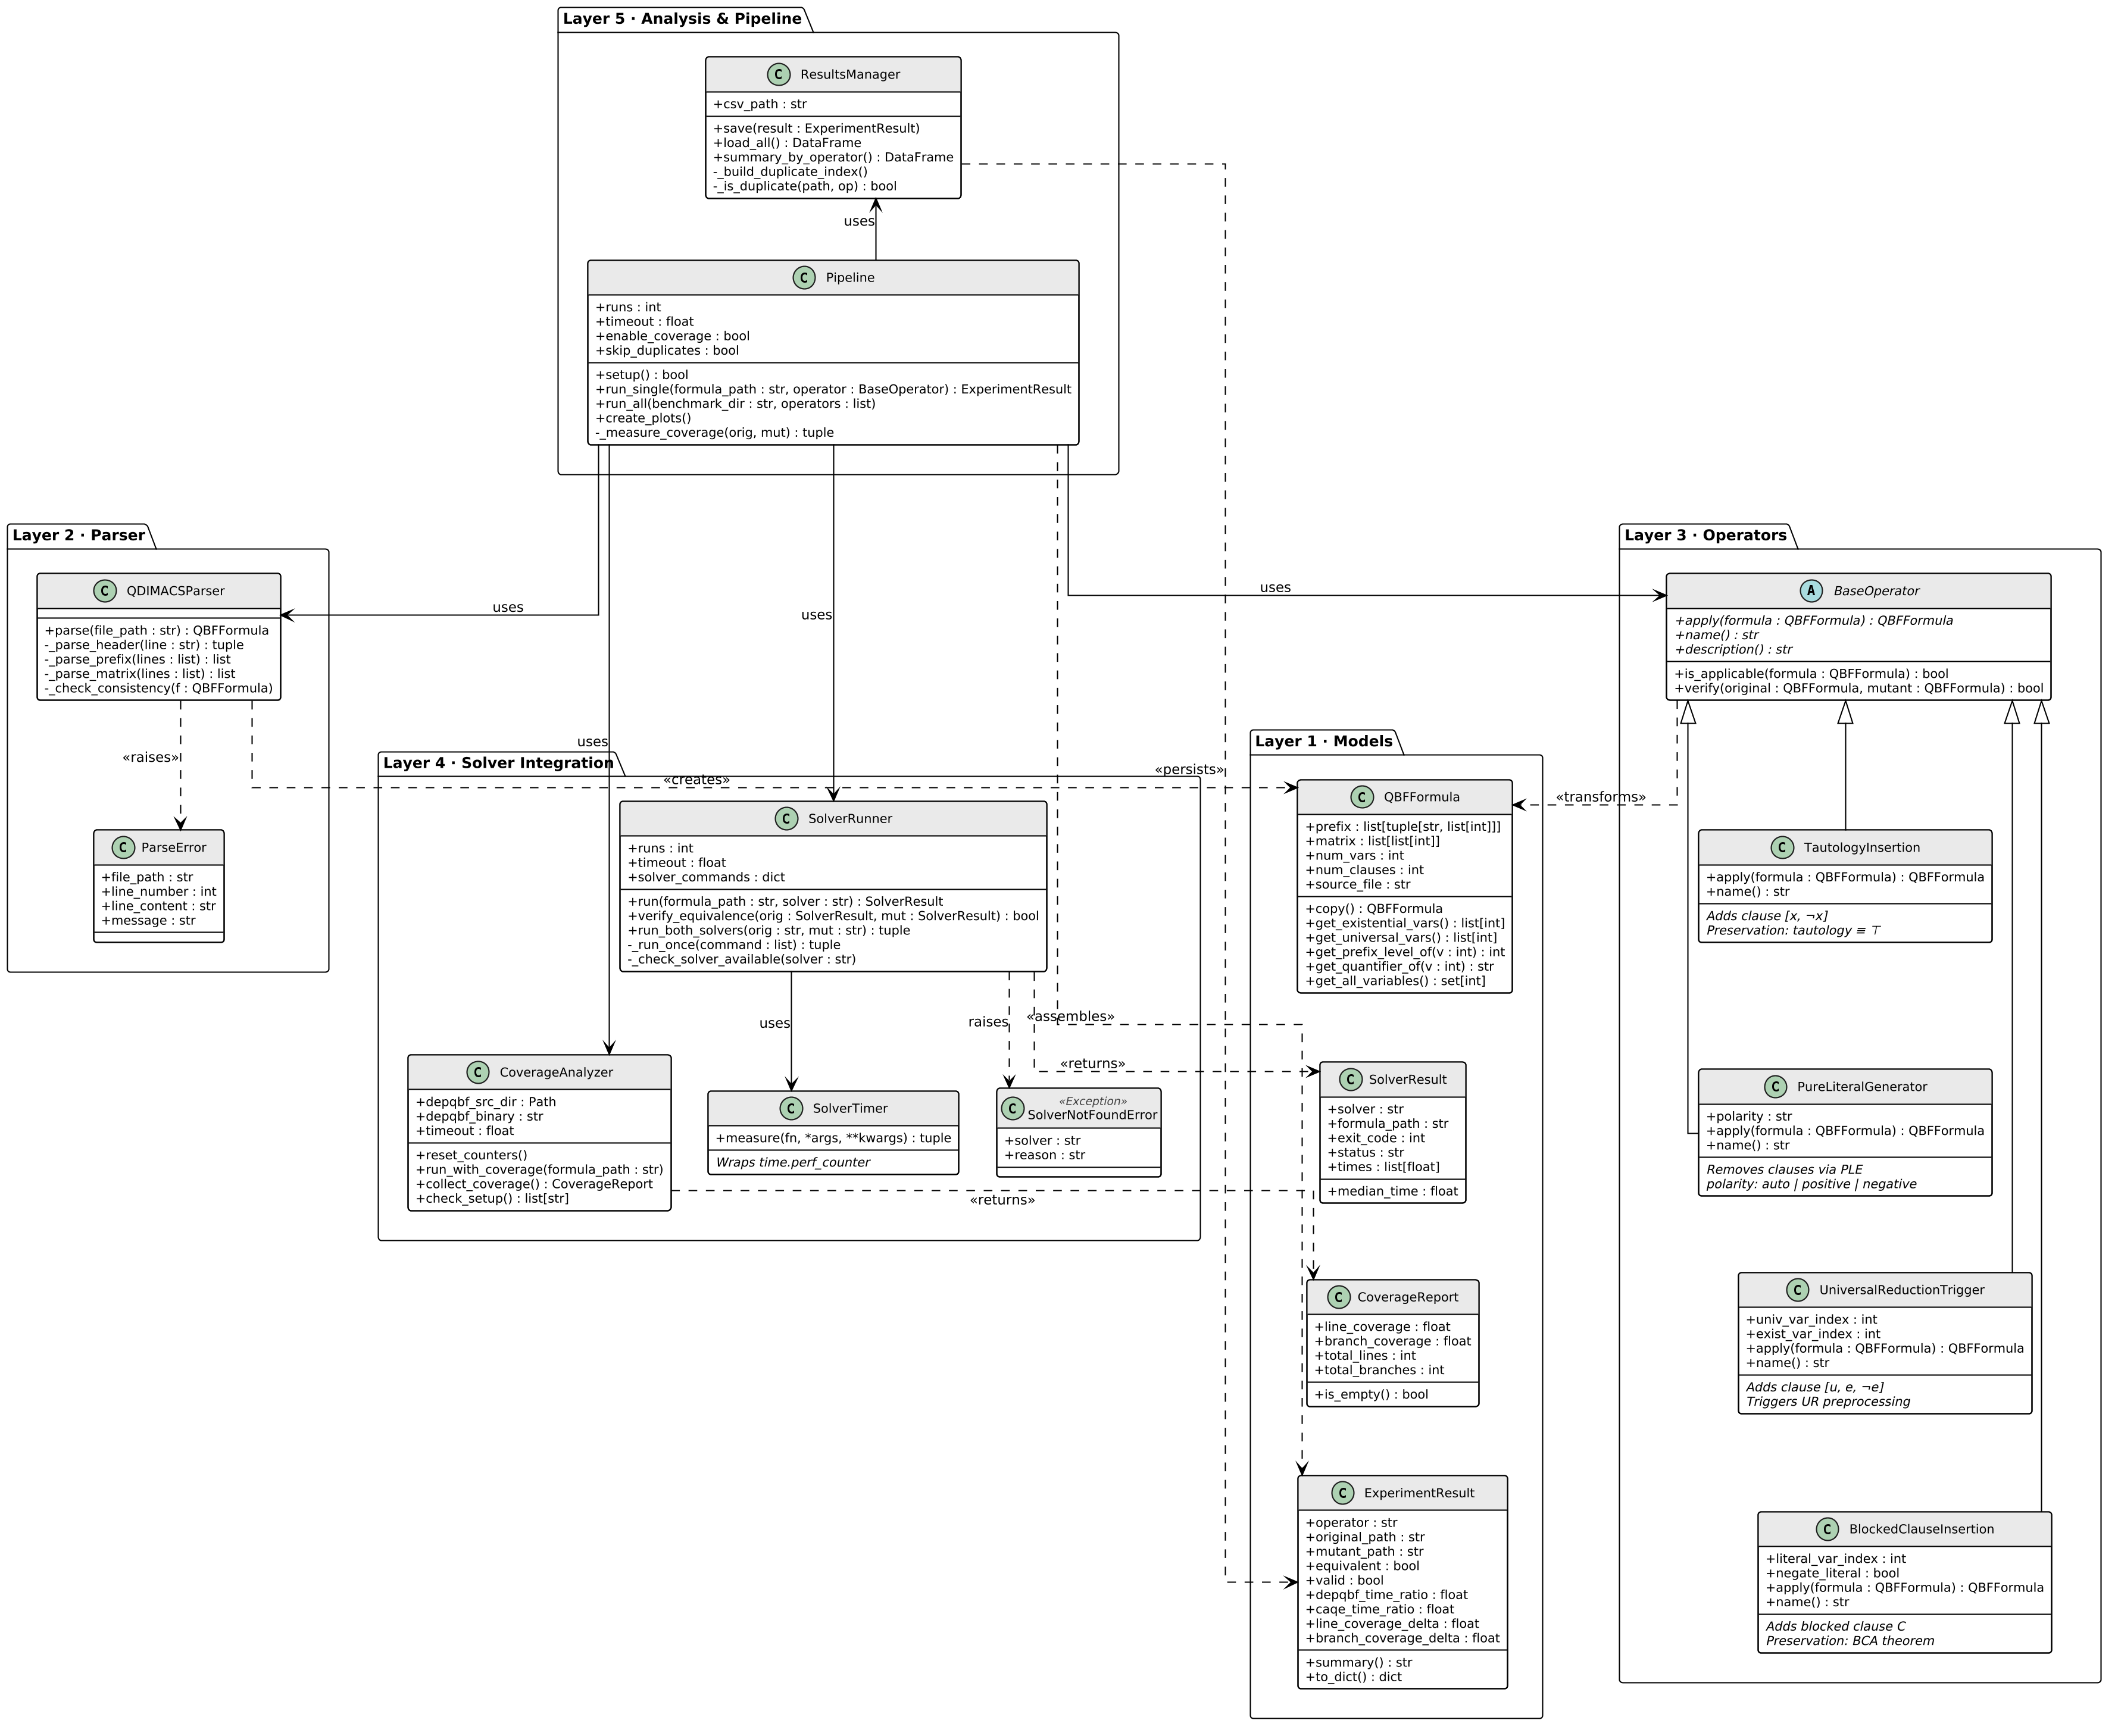
\includegraphics[width=\textwidth]{images/classDiagram.png}
  \caption{Class diagram of the QBF Transformer tool.}
  \label{fig:classdiagram}
\end{figure}

\section{Architecture Overview}\label{sec:architecture}

The system is structured into five layers that correspond directly to the five steps of the experimental pipeline:

\begin{enumerate}
  \item \textbf{Models} --- data classes that represent the domain objects: \texttt{QBFFormula}, \texttt{SolverResult}, \texttt{CoverageReport}, and \texttt{ExperimentResult}.
  \item \textbf{Parser} --- the \texttt{QDIMACSParser} and \texttt{ParseError} classes, which read \texttt{.qdimacs} files and validate their structure.
  \item \textbf{Operators} --- the \texttt{BaseOperator} abstract class and its four concrete subclasses, one per transformation.
  \item \textbf{Solver integration} --- \texttt{SolverTimer}, \texttt{SolverRunner}, and \texttt{CoverageAnalyzer}, which invoke the external solvers and collect measurements.
  \item \textbf{Analysis and pipeline} --- \texttt{ResultsManager}, the \texttt{Pipeline} class in \texttt{main.py}, which orchestrate the full experiment loop and persist results, and a Jupyter notebook(\texttt{\seqsplit{qbf\_solver\_analysis\_notebook.ipynb}}), 
        located in the project root directory, for interactive plot generation and data analysis.

\end{enumerate}

The dependency direction is strictly top-down: each layer uses only 
the layer below it, and no circular dependencies exist between 
modules. An additional utility script, \texttt{filter\_benchmarks.py}, 
is provided outside the main pipeline to select suitable benchmark formulas 
from the QBFLIB repository by filtering on variable count, clause count, 
and prefix-block count; it was used to produce the 50 
benchmark formulas evaluated in Chapter~\ref{cha:evaluation}.

\section{Parser}\label{sec:parser}

The \texttt{QDIMACSParser} class reads a \texttt{.qdimacs} file line by line and constructs a \texttt{QBFFormula} object. Parsing proceeds in four stages:

\begin{enumerate}
  \item \textbf{Comment and blank line removal.} Lines beginning with \texttt{c} and empty lines are discarded. All remaining lines are kept with their original line numbers for error reporting.
  \item \textbf{Header parsing.} The first non-comment line must match the pattern \texttt{p cnf <num\_vars> <num\_clauses>}. Both integers are validated to be positive.
  \item \textbf{Prefix parsing.} Consecutive lines beginning with \texttt{a} (universal) or \texttt{e} (existential) are parsed into a list of \texttt{(quantifier, variables)} tuples. Each line must be terminated by \texttt{0}.
  \item \textbf{Matrix parsing.} The remaining lines are parsed as clauses. Each clause is a list of non-zero signed integers terminated by \texttt{0}.
\end{enumerate}

After parsing, a consistency check verifies that the number of parsed clauses matches \texttt{num\_clauses} from the header, and that every variable referenced in the matrix appears in the prefix. Any violation raises a \texttt{ParseError} that includes the file path, line number, and offending line content, enabling precise diagnosis.

\section{Operator Design}\label{sec:operators-impl}

All four transformation operators share a common interface defined by the abstract base class \texttt{BaseOperator}. The class enforces the \emph{Template Method} pattern: subclasses must implement three abstract methods and may override two optional ones.

\begin{description}
  \item[\texttt{apply(formula)}] Applies the transformation and returns a new \texttt{QBFFormula} object. The original formula must never be modified; the method always calls \texttt{formula.copy()} before making any changes.
  \item[\texttt{name()}] Returns a unique, machine-readable identifier string (e.g.\ \texttt{"tautology\_insertion"}), used as a column value in the CSV output and as a file-name suffix for mutants.
  \item[\texttt{description()}] Returns a human-readable explanation of the transformation.
  \item[\texttt{is\_applicable(formula)}] (optional) Returns \texttt{True} if the preconditions for the operator are met. For example, \texttt{UniversalReductionTrigger} requires at least one universal variable $u$ and one existential variable $e$ with $\mathrm{level}(u) < \mathrm{level}(e)$ (see Section~\ref{sec:ur}). If \texttt{is\_applicable} returns \texttt{False}, the pipeline skips the experiment rather than raising an error.
  \item[\texttt{verify(original, mutant)}] (optional) Performs a post-hoc structural sanity check. This is not a full equivalence proof --- that role is played by the solvers --- but a fast check that the transformation was carried out as intended (e.g.\ the mutant has exactly one more clause than the original).
\end{description}

The eight operator instances registered in \texttt{main.py} are:

\begin{itemize}
  \item \texttt{TautologyInsertion()}
  \item 
    \texttt{\seqsplit{PureLiteralGenerator(polarity="auto")}}, 
    \texttt{\seqsplit{PureLiteralGenerator(polarity="positive")}}, 
    \texttt{\seqsplit{PureLiteralGenerator(polarity="negative")}}
  \item \texttt{UniversalReductionTrigger()}
  \item \texttt{BlockedClauseInsertion()}, 
    \texttt{BlockedClauseInsertion(negate\_literal=True)}, 
    \texttt{BlockedClauseInsertion(literal\_var\_index=1)}
\end{itemize}


Each variant has a distinct \texttt{name()} return value, ensuring that 
results from different configurations of the same operator are stored as 
separate rows in the CSV. 
For \texttt{BlockedClauseInsertion}, the suffix \texttt{\_neg} is appended when 
\texttt{negate\_literal=True}, and the suffix \texttt{\_v\{index\}} is appended when \texttt{literal\_var\_index} 
is non-zero; thus \texttt{\seqsplit{BlockedClauseInsertion(literal\_var\_index=1)}} 
produces the name \texttt{blocked\_clause\_insertion\_v1}.

\section{Solver Integration}\label{sec:solver-impl}

\subsection{SolverTimer and SolverRunner}

Runtime measurement is handled by \texttt{SolverTimer}, which wraps each solver invocation with \texttt{time.perf\_counter}. This clock is monotonic and unaffected by system time corrections, making it suitable for high-resolution process timing.

\texttt{SolverRunner} invokes the external solver binaries via Python's \texttt{subprocess} module. Each solver is called with the path to the formula file as a command-line argument:

\begin{listing}[H]
\caption{Solver invocation commands.}
\label{lst:solver-calls}
\begin{minted}[frame=single,fontsize=\small]{text}
# DepQBF
depqbf --qdo <formula.qdimacs>

# CAQE
caqe <formula.qdimacs>
\end{minted}
\end{listing}

The solver's exit code is interpreted according to the QDIMACS convention: 
exit code \texttt{10} maps to \texttt{SAT}, exit code \texttt{20} maps to 
\texttt{UNSAT}, and any other exit code (including timeout) is recorded as 
\texttt{ERROR}. Each formula is solved once per experiment. Since the primary 
research focus is on correctness (equivalence preservation) and code coverage 
rather than on precise performance benchmarking, a single run is sufficient to 
detect operator-specific differences in solver behavior. The reported runtime 
is the wall-clock time of that run.

The \emph{runtime ratio} for a single experiment is defined as:
\[
  \text{ratio} = \frac{\text{time}(\text{mutant})}{\text{time}(\text{original})}.
\]
A ratio greater than $1.0$ indicates that the mutant takes longer to solve; a ratio less than $1.0$ indicates that the mutant is solved faster.

\subsection{Equivalence Verification}\label{sec:equivalence-verification-impl}

After both the original and the mutant have been solved, 
\texttt{SolverRunner} checks that the results are consistent. 
An experiment is marked \texttt{equivalent = True} if and only 
if the status of the original and the status of the mutant are 
identical (both SAT or both UNSAT) for \textbf{DepQBF}. The CAQE 
results are recorded in the CSV and can be inspected post-hoc, 
but are not used as part of the formal equivalence flag. Any 
discrepancy in the DepQBF results is flagged as a truth-value 
violation and excluded from the runtime and coverage analysis.

\section{Coverage Analysis}\label{sec:coverage-impl}

Code coverage is measured using \texttt{gcov}, which requires DepQBF to be compiled with GCC instrumentation flags:

\begin{listing}[H]
\caption{DepQBF instrumented build command.}
\label{lst:gcov-build}
\begin{minted}[frame=single,fontsize=\small]{bash}
make CFLAGS="-fprofile-arcs -ftest-coverage -O0"
\end{minted}
\end{listing}

The \texttt{CoverageAnalyzer} class implements a three-step measurement protocol for each formula:

\begin{enumerate}
  \item \textbf{Reset.} All \texttt{.gcda} files in the DepQBF source directory are deleted. This clears the execution counters from any previous run.
  \item \textbf{Execute.} DepQBF is invoked once on the formula via \texttt{subprocess}. The instrumented binary writes \texttt{.gcda} files recording which basic blocks were executed and how many times.
  \item \textbf{Collect.} \texttt{gcov} is called on the DepQBF source files. Its standard output contains lines of the form \texttt{Lines executed: X\% of N} and \texttt{Branches executed: Y\% of M}, which are extracted by the \texttt{CoverageAnalyzer} parser and stored in a \texttt{CoverageReport} object.
\end{enumerate}

This protocol is executed twice per experiment: once for the original formula and once for the mutant. The coverage delta is then computed as:
\[
  \Delta_{\text{line}} = \text{line\_coverage}(\text{mutant}) - \text{line\_coverage}(\text{original}),
\]
and analogously for branch coverage. A positive delta indicates that the mutant caused the solver to traverse additional code paths.

\textbf{Platform note.} On macOS, Apple Clang does not support \texttt{gcov} instrumentation. The instrumented DepQBF binary must therefore be compiled with \texttt{gcc-15} installed via Homebrew, and the \texttt{gcov} binary must be explicitly set to \texttt{gcov-15}.

\section{Pipeline and Result Persistence}\label{sec:pipeline-impl}

The \texttt{Pipeline} class in \texttt{main.py} orchestrates the complete experimental loop. Its \texttt{run\_all()} method iterates over every combination of benchmark formula and operator, calling \texttt{run\_single()} for each pair. The \texttt{run\_single()} method executes the five pipeline steps in sequence:

\begin{enumerate}
  \item Parse the original formula with \texttt{QDIMACSParser}.
  \item Apply the operator to produce a mutant and write it to disk as a \texttt{.qdimacs} file.
  \item Run both solvers on original and mutant with \texttt{SolverRunner}.
  \item Measure coverage for both with \texttt{CoverageAnalyzer}.
  \item Assemble an \texttt{ExperimentResult} and persist it via \texttt{ResultsManager}.
\end{enumerate}

\texttt{ResultsManager} appends each result immediately to a CSV file using \texttt{pandas}. 
All plots and statistical summaries are produced separately in the Jupyter notebook \texttt{qbf\_solver\_analysis\_\allowbreak notebook.ipynb}, which loads the CSV and generates the figures used in Chapter~\ref{cha:evaluation}. 
Writing incrementally rather than in batch ensures that no data is lost if the pipeline is interrupted. 
A duplicate detection mechanism based on an in-memory set (keyed on formula path, operator name, and mutant path) prevents re-running experiments that are already present in the CSV, enabling the pipeline to be resumed after interruption in $O(1)$ per lookup.

The CSV schema contains one row per experiment with the following columns: \texttt{operator}, \texttt{original\_path}, \texttt{mutant\_path}, \texttt{equivalent}, \texttt{valid}, solver status and median time 
for both solvers on both formulas, the runtime ratio for each solver, and line and branch coverage for original, mutant, and their delta. This flat structure is directly consumed by the Jupyter notebook described in Chapter~\ref{cha:evaluation}.

\section{Command-Line Interface}\label{sec:cli}

The tool is invoked from the command line via \texttt{main.py}. The most common usage patterns are:

\begin{listing}[H]
\caption{CLI usage examples.}
\label{lst:cli}
\begin{minted}[frame=single,fontsize=\small]{bash}
# Run all formulas x all operators
python main.py

# Run one specific formula
python main.py --formula benchmarks/formula_001.qdimacs

# Run one specific operator only
python main.py --operator tautology_insertion

# Adjust run count and timeout
python main.py --timeout 30

# Disable coverage measurement (faster)
python main.py --no-coverage

# Generate summary from existing CSV (no new experiments)
python main.py --plots-only
\end{minted}
\end{listing}

Additional configuration arguments control solver binary paths 
(\texttt{--depqbf-src}, \texttt{--depqbf-binary}), the output 
CSV path (\texttt{--results-csv}), the benchmark directory 
(\texttt{--benchmark-dir}), and duplicate detection behaviour (\texttt{--no-skip-duplicates}, which disables the duplicate check and forces re-running all experiments). 
By default, the pipeline skips formula--operator combinations that are already present in the 
CSV, enabling interrupted runs to be resumed without recomputing 
existing results.

%%% Local Variables:
%%% tex-command: "pdflatex"
%%% TeX-master: "../main"
%%% TeX-command-extra-options: "-shell-escape"
%%% End:
\chapter{Evaluation}\label{cha:evaluation}

This chapter presents the experimental results of the QBF Transformer tool. 
Section~\ref{sec:setup} describes the experimental setup, and Section~\ref{sec:equivalence-verification} verifies the correctness of the transformations via the equivalence rate. Sections~\ref{sec:runtime}--\ref{sec:secondary} present the measurements for runtime, coverage, and the relationship between coverage change and runtime effect. Section~\ref{sec:eval-summary} summarises all results in a single table.

\section{Experimental Setup}\label{sec:setup}

\subsection{Benchmark Formulas}\label{sec:benchmarks}

The experiments were conducted on a set of 50 QBF benchmark formulas in
QDIMACS format, drawn from the QBFLIB repository (Basler, Castellini,
Jordan-Kaiser, Kronegger-Pfandler-Pichler, Tacchella, Tentrup, and
Wintersteiger benchmark families).
Formulas were selected using the \texttt{filter\_benchmarks.py} utility,
retaining only instances that satisfy all of the following criteria:
\begin{itemize}
  \item at most 200 variables,
  \item at most 1\,000 clauses,
  \item at least two quantifier prefix blocks, and
  \item at least one universal and at least one existential quantifier block
        (formulas with only a single quantifier type are excluded as trivial).
\end{itemize}
 
A total of 400 experiments were recorded across all operator and formula
combinations (50 formulas $\times$ 8 operators).
After filtering for operator applicability, 285 experiments were retained
for analysis.
The equivalence rate and the reasons for exclusion are discussed in
Section~\ref{sec:equivalence-verification}.


\subsection{Operators and Variants}\label{sec:operators}

Eight operator variants were evaluated, grouped into four families:
 
\begin{itemize}
  \item \textbf{Tautology Insertion} (1 variant):
        \texttt{tautology\_insertion}
  \item \textbf{Pure Literal Generator} (3 variants, differing in
        which polarity of pure literal is selected):
        \texttt{pure\_literal\_gen\_auto} (any polarity),
        \texttt{pure\_literal\_gen\_pos} (positive only),
        \texttt{pure\_literal\_gen\_neg} (negative only)
  \item \textbf{Universal Reduction Trigger} (1 variant):
        \texttt{universal\_reduction\_trigger}
  \item \textbf{Blocked Clause Insertion} (3 variants, differing in the blocking-literal selection):
        \texttt{\seqsplit{blocked\_clause\_insertion}} (first existential, positive),
        \texttt{blocked\_clause\_insertion\_neg} (first existential, negated),
        \texttt{blocked\_clause\_insertion\_v1} (second existential)
\end{itemize}

\subsection{Measurement Parameters}\label{sec:measurement}

Each formula was solved once per solver per experiment. As the focus of this 
thesis is correctness verification and coverage analysis rather than fine-grained 
performance benchmarking, a single run is adequate to capture operator-specific 
effects. A per-experiment timeout of 60 seconds was applied. 
Runtime was measured with \texttt{time.perf\_counter}; code coverage was
collected via \texttt{gcov} on an instrumented build of DepQBF compiled
with \texttt{gcc-15}.


\subsection{Equivalence Verification}\label{sec:equivalence-verification}

Before analysing runtime and coverage, the correctness of each transformation
must be verified.
An experiment is marked as \emph{equivalent} if and only if DepQBF returns
the same result (SAT or UNSAT) for both the original and the mutant
formula (see Section~\ref{sec:equivalence-verification-impl}).
CAQE results were additionally recorded and showed no discrepancies when
inspected post-hoc, but are not used as part of the formal equivalence flag.

Of 400 total experiments, 285 (71.25\%) produced valid results and were
retained for runtime and coverage analysis.
The remaining 115 experiments were excluded for two reasons:


\begin{itemize}
  \item \textbf{Operator non-applicability} (99 experiments): the Pure
        Literal Generator variants could not be applied to formulas
        that contained no pure literals.
  \item \textbf{Parse errors} (16 experiments): two benchmark files
        (\texttt{p10-1.pddl\_planlen=0} and
        \texttt{p5-5.pddl\_planlen=0}) contained an empty quantifier
        block (\texttt{e~0}), which is non-standard QDIMACS and caused
        a parse error in the tool
        ($2~\text{files} \times 8~\text{operators} = 16~\text{experiments}$).
\end{itemize}

Crucially, all 285 retained experiments achieved a 100\% equivalence rate:
DepQBF returned identical results (SAT or UNSAT) for every
original--mutant pair, confirming that all four transformation operators
are correctly implemented and truth-value-preserving in practice.

Figure~\ref{fig:equivalence} shows the equivalence rate per operator.
Operators for which all experiments were retained (Tautology Insertion,
Universal Reduction Trigger, and all Blocked Clause variants) show a bar
at 100\% with $n = 48$.
The Pure Literal Generator variants show lower $n$ values (19, 13, 13)
reflecting the cases where the operator was not applicable.

\begin{figure}[h]
  \centering
  
\includegraphics[width=\textwidth]{images/equivalence_rate.png}
  \caption{%
    Equivalence rate per transformation operator.
    The dashed green line marks the 100\% target.
    Bar labels show the equivalence rate and sample count~$n$.
    Operators with $n < 48$ were not applicable to all benchmark
    formulas (see text).%
  }
  \label{fig:equivalence}
\end{figure}

\section{Runtime Analysis}\label{sec:runtime}

The runtime effect of a transformation is quantified by the runtime ratio:
\[
  \text{ratio} = \frac{\text{median\_time}(\text{mutant})}{\text{median\_time}(\text{original})}.
\]
A ratio of $1.0$ indicates no change; values above $1.0$ indicate the mutant is slower; values below $1.0$ indicate the mutant is faster.

\subsection{Runtime Ratio per Operator — DepQBF}

Figure~\ref{fig:ratio-depqbf} shows the distribution of runtime ratios for DepQBF across all operators.

\begin{figure}[h]
  \centering
  
\includegraphics[width=\textwidth]{images/time_ratio_boxplot_depqbf.png}
  \caption{Runtime ratio (mutant / original) per operator for DepQBF. The dashed red line marks ratio~$= 1.0$.}
  \label{fig:ratio-depqbf}
\end{figure}

\subsection{Runtime Ratio per Operator — CAQE}

Figure~\ref{fig:ratio-caqe} shows the same distribution for CAQE.

\begin{figure}[h]
  \centering
  
\includegraphics[width=\textwidth]{images/time_ratio_boxplot_caqe.png}
  \caption{Runtime ratio (mutant / original) per operator for CAQE. The dashed red line marks ratio~$= 1.0$.}
  \label{fig:ratio-caqe}
\end{figure}

\subsection{Solver Comparison: DepQBF vs.\ CAQE}

Figure~\ref{fig:solver-comparison} directly compares the median runtime ratio of DepQBF and CAQE for each operator. Operators where both bars are on the same side of $1.0$ suggest a general structural effect; operators where the bars diverge suggest a solver-specific implementation effect.

\begin{figure}[h]
  \centering
  
\includegraphics[width=\textwidth]{images/solver_comparison.png}
  \caption{Median runtime ratio comparison between DepQBF and CAQE per operator.}
  \label{fig:solver-comparison}
\end{figure}

\subsection{Interpretation}

The Tautology Insertion operator produces a median runtime ratio of 
$0.990$ for DepQBF and $0.999$ for CAQE, both close to~$1.0$. The values 
fall just below~$1.0$, consistent with measurement noise at this scale, 
and confirm that adding a trivially discarded clause causes only minimal overhead.
The Pure Literal Generator variants consistently show ratios below $1.0$ for DepQBF 
(auto: $0.968$, positive: $0.976$, negative: $0.980$), consistent with the prediction 
that eliminating clauses reduces the formula size and accelerates DepQBF. 
For CAQE the corresponding ratios are essentially at $1.0$ (auto: $1.002$, 
positive: $1.003$, negative: $0.999$), suggesting that the size reduction has 
a much weaker effect on CAQE's clausal-abstraction strategy than on DepQBF's 
search-based procedure. The Universal Reduction Trigger shows a small but 
notable solver asymmetry: $0.988$ for DepQBF (mutant slightly faster) 
versus $1.005$ for CAQE (mutant slightly slower), suggesting that 
DepQBF benefits marginally from the inserted clause being simplified 
away during preprocessing, while CAQE incurs a small overhead from 
the additional clause. The Blocked Clause Insertion variants show 
ratios slightly below $1.0$ for DepQBF ($0.988$--$0.992$), and ratios 
slightly above $1.0$ for CAQE ($1.002$--$1.005$), consistent with 
the same solver asymmetry and the formula-structure dependence of 
blocked clause detection.

\section{Coverage Analysis}\label{sec:coverage}

Code coverage is measured as the percentage of DepQBF source lines and branches
executed during solving. The coverage delta~$\Delta$ is defined as:
\[
  \Delta = \text{coverage}(\text{mutant}) - \text{coverage}(\text{original}).
\]
A positive delta indicates that the mutant formula caused the solver to execute
additional code; a negative delta indicates that fewer code paths were reached.
Coverage was collected only for DepQBF, as \texttt{gcov} instrumentation is not
available for the CAQE binary.

\subsection{Line Coverage Delta}

Figure~\ref{fig:coverage-line} shows the median line coverage delta per operator.
Error bars represent the interquartile range~(IQR) across all experiments in that
operator group.

\begin{figure}[h]
  \centering
  
\includegraphics[width=\textwidth]{images/coverage_delta_line.png}
  \caption{%
    Line coverage delta ($\Delta$ line coverage in percentage points,~pp) per
    operator. Bars show the median; error bars show the interquartile range~(IQR).
    Positive values indicate the mutant activates additional source lines in DepQBF.%
    }
  \label{fig:coverage-line}
\end{figure}

\subsection{Branch Coverage Delta}

Figure~\ref{fig:coverage-branch} shows the median branch coverage delta per operator.
Branch coverage is strictly finer than line coverage: a single \texttt{if}-statement
contributes two branches, so branch deltas tend to be slightly larger in magnitude
than the corresponding line deltas.

\begin{figure}[h]
  \centering
  
\includegraphics[width=\textwidth]{images/coverage_delta_branch.png}
  \caption{%
    Branch coverage delta ($\Delta$ branch coverage in percentage points,~pp) per
    operator. Bars show the median; error bars show the interquartile range~(IQR).
    Positive values indicate the mutant causes additional conditional branches to be
    taken in DepQBF.%
     }
  \label{fig:coverage-branch}
\end{figure}

\subsection{Interpretation}\label{sec:coverage-interpretation}

\textbf{Tautology Insertion} produces a median line coverage delta of
$+0.033\,\text{pp}$ and a branch delta of $+0.030\,\text{pp}$.
Both values are positive, indicating that the inserted tautological clause
$(\ell \lor \neg\ell)$ triggers an additional preprocessing code path in DepQBF
that is not reached by the original formula.
 
\textbf{Pure Literal Generator} (all three variants: auto, positive, negative)
consistently produce negative deltas of $-0.017\,\text{pp}$ (line) and
$-0.030\,\text{pp}$ (branch).
This is consistent with the design intent of this operator: by applying Pure Literal
Elimination to produce a strictly smaller mutant, the transformed formula traverses
fewer solver-internal code paths than the original. All three variants produce
identical coverage deltas because they share the same elimination mechanism and
differ only in which pure literal is selected.

\textbf{Universal Reduction Trigger} produces a median line delta of
$+0.033\,\text{pp}$ and branch delta of $+0.030\,\text{pp}$, identical to
Tautology Insertion.
This suggests that the inserted clause $[u, e, \neg e]$ activates the same
preprocessing code path as the tautological clause — consistent with the
expectation that Universal Reduction is applied during the same preprocessing
phase as tautology detection.
 
\textbf{Blocked Clause Insertion} (Standard variant) produces a median line
delta of $+0.017\,\text{pp}$ and branch delta of $+0.015\,\text{pp}$,
approximately half the delta of Tautology Insertion. This suggests partial
activation of the blocked clause detection code path.
 
\textbf{Blocked Clause (Negated)} produces the largest positive delta of all
operators: $+0.075\,\text{pp}$ line and $+0.091\,\text{pp}$ branch. The larger
delta compared to the standard variant suggests that negating the blocking literal
activates a different, less frequently reached branch within the blocked clause
detection routine of DepQBF.
 
\textbf{Blocked Clause (Variant~2)} produces a delta of exactly $0\,\text{pp}$
for both line and branch coverage. The inserted clause is handled by an
already-covered code path, meaning no new lines or branches are reached by the mutant.

It is noteworthy that the Blocked Clause (Negated) and Blocked Clause (Standard)
variants exhibit large IQR error bars (approximately $\pm 0.5\,\text{pp}$),
reflecting high variability across benchmark formulas. This variability is
formula-structure-dependent: blocked clause detection is only triggered when the
inserted clause is blocked with respect to the formula's existing clause set,
which varies per instance.

\section{Secondary Analysis: Coverage Change vs.\ Runtime Effect}\label{sec:secondary}

This section investigates whether a larger coverage delta is associated with a larger runtime ratio. Figures~\ref{fig:cov-vs-ratio-depqbf} and~\ref{fig:cov-vs-ratio-caqe} provide an overview across both solvers: each point represents one experiment, with the coverage delta on the $x$-axis and the runtime ratio on the $y$-axis. Points are colour-coded by operator family.

\begin{figure}[h]
  \centering
  
\includegraphics[width=\textwidth]{images/scatter_depqbf.png}
  \caption{Coverage delta (pp) vs.\ runtime ratio for DepQBF. The dashed red line marks ratio $= 1.0$.}
  \label{fig:cov-vs-ratio-depqbf}
\end{figure}

\begin{figure}[h]
  \centering
  
\includegraphics[width=\textwidth]{images/scatter_caqe.png}
  \caption{Coverage delta (pp) vs.\ runtime ratio for CAQE. The dashed red line marks ratio $= 1.0$.}
  \label{fig:cov-vs-ratio-caqe}
\end{figure}

Figure~\ref{fig:coverage-vs-ratio} then breaks the DepQBF data down by operator family, with a linear trend line with slope $m$ fitted per group.

\begin{figure}[h]
  \centering
  
\includegraphics[width=\textwidth]{images/coverage_vs_ratio_depqbf.png}
  \caption{Coverage delta (pp) vs.\ runtime ratio for DepQBF, grouped by operator family. The dashed coloured line shows a linear fit with slope $m$; the dotted red line marks ratio $= 1.0$.}
  \label{fig:coverage-vs-ratio}
\end{figure}

For three of the four operator groups the fitted slope is close to zero
($|m| \leq 0.074$), indicating no meaningful linear relationship between
coverage delta and runtime ratio.
The exception is \textbf{Tautology Insertion} ($m = -0.472$): a larger
positive coverage delta is weakly associated with a \emph{lower} runtime
ratio, suggesting that reaching additional preprocessing code paths
slightly reduces solving time rather than increasing it.
However, the Tautology Insertion group spans a narrow coverage range
(approximately $-0.01$ to $+0.03\,\text{pp}$) with few distinct delta
values, so this slope should not be over-interpreted.

The \textbf{Blocked Clause Addition} group exhibits the widest spread on
both axes: coverage deltas range from approximately $-1\,\text{pp}$ to
$+3\,\text{pp}$, and runtime ratios range from roughly $0.75$ to $1.25$.
Despite this spread, the slope is nearly flat ($m = 0.003$), confirming
that coverage delta is not a predictor of runtime change within this group.
The large variance is consistent with the formula-structure dependence of
blocked clause detection noted in Section~\ref{sec:coverage-interpretation}.

Overall, the analysis provides no evidence that a larger coverage delta
causes a larger runtime effect across any operator group.

\section{Summary}\label{sec:eval-summary}

\begin{table}[h]
\centering
\caption{Aggregated results per transformation operator (n = number of valid experiments; ratios and coverage deltas are medians across formulas).}
\label{tab:summary}
\resizebox{\textwidth}{!}{%
\begin{tabular}{llrrrrr}
\toprule
\textbf{Operator} & \textbf{Group} & \textbf{n} &
\textbf{Ratio DepQBF} & \textbf{Ratio CAQE} &
\textbf{$\Delta$ Line (pp)} & \textbf{$\Delta$ Branch (pp)} \\
\midrule
\texttt{tautology\_insertion}            & Tautology           & 48 & $0.990$ & $0.999$ & $+0.033$ & $+0.030$ \\
\texttt{pure\_literal\_gen\_auto}        & Pure Literal        & 19 & $0.968$ & $1.002$ & $-0.017$ & $-0.030$ \\
\texttt{pure\_literal\_gen\_pos}         & Pure Literal        & 13 & $0.976$ & $1.003$ & $-0.017$ & $-0.030$ \\
\texttt{pure\_literal\_gen\_neg}         & Pure Literal        & 13 & $0.980$ & $0.999$ & $-0.017$ & $-0.030$ \\
\texttt{universal\_reduction\_trigger}   & Universal Reduction & 48 & $0.988$ & $1.005$ & $+0.033$ & $+0.030$ \\
\texttt{blocked\_clause\_insertion}      & Blocked Clause      & 48 & $0.988$ & $1.005$ & $+0.017$ & $+0.015$ \\
\texttt{blocked\_clause\_insertion\_neg} & Blocked Clause      & 48 & $0.992$ & $1.002$ & $+0.075$ & $+0.091$ \\
\texttt{blocked\_clause\_insertion\_v1}  & Blocked Clause      & 48 & $0.989$ & $1.004$ & $+0.000$ & $+0.000$ \\
\bottomrule
\end{tabular}}
\end{table}

All DepQBF runtime ratios fall within the range $0.968$--$0.992$, confirming
that none of the transformations causes measurable overhead for DepQBF\@.
The Pure Literal Generator variants produce the lowest DepQBF ratios
($0.968$--$0.980$), consistent with the expectation that a smaller mutant
formula reduces solving time.

For CAQE, the picture is reversed for several operators: Universal Reduction,
Blocked Clause (Standard), and Blocked Clause (Variant~2) all show CAQE ratios
slightly above $1.0$ ($1.004$--$1.005$), meaning the mutant is marginally
\emph{slower} for CAQE\@. This solver-specific asymmetry suggests that the two
solvers handle the inserted clauses differently during preprocessing: DepQBF
appears to simplify them away at a net benefit, while CAQE incurs a small
overhead.

Coverage deltas remain small across all operators (below $0.10\,\text{pp}$
in all cases), reflecting the limited size of the benchmark formulas.
The Blocked Clause (Negated) variant produces the largest positive delta
($+0.075\,\text{pp}$ line, $+0.091\,\text{pp}$ branch), suggesting that
negating the blocking literal activates additional preprocessing code paths
in DepQBF\@. The Pure Literal Generator variants consistently produce negative
deltas ($-0.017\,\text{pp}$ line, $-0.030\,\text{pp}$ branch); the three
variants yield identical deltas because they share the same elimination
mechanism and differ only in which pure literal is selected. A smaller
mutant formula causes the solver to traverse fewer code paths overall.
\chapter{Conclusion}\label{cha:conclusion}

\section{Summary of Contributions}\label{sec:summary}

This thesis investigated whether truth-value-preserving
transformations can be used to systematically test QBF solvers by
deliberately activating specific internal mechanisms while
preserving the correct solver output as an oracle. To this end, the
\emph{QBF Transformer} tool was designed and implemented as a
complete experimental pipeline covering parsing, transformation,
solving with DepQBF and CAQE, runtime measurement, and \texttt{gcov}
coverage analysis.

Four operators were formally defined and proven truth-value-preserving
(see Chapter~\ref{cha:operators}): \emph{Tautology Insertion},
\emph{Pure Literal Generator}, \emph{Universal Reduction Trigger},
and \emph{Blocked Clause Insertion}. Each operator targets a
distinct internal solver mechanism.

The empirical evaluation over 285 valid experiments achieved a
100\,\% equivalence rate, confirming that all four operators are
correctly implemented in practice. The aggregated measurements
(Table~\ref{tab:summary}) show that the operators produce
measurable, operator-specific effects on both runtime and coverage,
though the absolute magnitudes are small for the benchmark set
used. A consistent asymmetry between the two solvers emerged:
DepQBF shows runtime ratios at or below~$1.0$ across all operators,
whereas CAQE shows ratios at or above~$1.0$ for most operators.
This suggests solver-specific differences in preprocessing that
warrant further investigation.

\section{Limitations}\label{sec:limitations}

\textbf{Benchmark size.} Only 50 formulas from seven QBFLIB
families were evaluated. The small absolute coverage deltas
(below~$0.10\,\text{pp}$) reflect the limited size of the
benchmarks rather than the absence of an effect; larger and more
diverse sets (e.g.\ the QBF Gallery) would be needed for
statistically robust conclusions.

\textbf{Coverage measurement limited to DepQBF.} \texttt{gcov} is
not directly applicable to CAQE's Rust build, so the runtime
asymmetry observed for CAQE cannot currently be explained at the
code-path level.

\textbf{Equivalence check via DepQBF only.} The equivalence flag
relies on DepQBF's output; a systematic DepQBF bug would not be
detected by this check alone.

\textbf{Structural transformations only.} All four operators are
syntactic. Semantic transformations exploiting dependency schemes
or quantifier-alternation depth could potentially activate deeper
solver code paths.


\section{Future Work}\label{sec:future}

Several directions follow naturally from this work.
\emph{Larger benchmark sets} from QBFLIB or the QBF Gallery would
enable statistically meaningful per-family comparisons.
\emph{Additional operators} could target clause learning
(Q-resolution), dependency scheme computation, or certificate
generation. \emph{Mutation testing} of the solver source itself
would quantify the sensitivity of the test method by checking
whether injected bugs are detected by the equivalence flag.
\emph{Automated operator synthesis} using constraint solving or
program synthesis could discover new truth-value-preserving
transformations beyond those designed by hand. Finally,
\emph{cross-solver coverage} via Rust-native tooling
(e.g.\ \texttt{cargo-llvm-cov}) would allow the DepQBF/CAQE runtime
asymmetry to be investigated symmetrically --- arguably the most
important open question left by this thesis.

%%%%%%%%%%%%%%%%%%
\printbibliography%

%%%%%%%%%
\appendix

%TODO if another pdf should be appended/added
%\includepdf[pages=-]{paper.pdf}

\end{document}

%%% Local Variables:
%%% TeX-engine: default
%%% TeX-master: t
%%% TeX-command-extra-options: "-shell-escape"
%%% End: